%
\documentclass{sig-alternate-10pt}
\usepackage{subfigure}
\usepackage{color}
\usepackage{authblk}
\usepackage{multirow}
\usepackage{times}
\usepackage{amsmath}
\usepackage{paralist}
%\usepackage{graphicx}
%\usepackage{amssymb}
%\usepackage{bm}
%\usepackage{ifthen}
%\usepackage{paralist}
%\usepackage{cite}
\usepackage{url}
%\usepackage{subfigure}
%\usepackage{threeparttable}
%%%%%%%%%%%% real, integer notation
\newcommand{\real}{{\mathbb R}}
\newcommand{\integer}{{\mathbb Z}}


% boldface characters
% macro by mung

\newcommand{\td}{\ensuremath{t_{\text{dl}}}}
\newcommand{\bx}{\bm{x}}
\newcommand{\bc}{\bm{c}}
\newcommand{\bbx}{\ensuremath{{\bm x}}}
\newcommand{\bbc}{\ensuremath{{\bm c}}}
\newcommand{\bu}{\ensuremath{{\bm u}}}

\newcommand{\bz}{\ensuremath{{\bm z}}}
\newcommand{\ba}{\ensuremath{{\bm a}}}
\newcommand{\be}{\ensuremath{{\bm e}}}
\newcommand{\br}{\ensuremath{{\bm r}}}
\newcommand{\by}{\ensuremath{{\bm y}}}
\newcommand{\bby}{\ensuremath{{\bm y}}}
\newcommand{\bbq}{\ensuremath{{\bm q}}}


\newcommand{\bp}{\ensuremath{{\bm p}}}
\newcommand{\bh}{\ensuremath{{\bm h}}}
\newcommand{\bP}{\bm{P}}
\newcommand{\bA}{\ensuremath{{\bm A}}}

\newcommand{\bF}{\bm{F}}
\newcommand{\bN}{\ensuremath{{\bm N}}}
\newcommand{\bbf}{\ensuremath{{\bm f}}}
\newcommand{\bG}{\ensuremath{{\bm G}}}
\newcommand{\bQ}{\ensuremath{{\bm Q}}}
\newcommand{\bH}{\ensuremath{{\bm H}}}
\newcommand{\bW}{\ensuremath{{\bm W}}}
\newcommand{\bJ}{\ensuremath{{\bm J}}}
\newcommand{\bg}{\ensuremath{{\bm g}}}
\newcommand{\bs}{\ensuremath{{\bm s}}}

\newcommand{\bbv}{\ensuremath{{\bm v}}}
\newcommand{\bbz}{\ensuremath{{\bm z}}}
\newcommand{\bbu}{\ensuremath{{\bm u}}}
\newcommand{\bbm}{\ensuremath{{\bm m}}}
\newcommand{\bbU}{\ensuremath{{\bm U}}}
\newcommand{\bw}{\bm{w}}
\newcommand{\bbr}{\ensuremath{{\bm r}}}
\newcommand{\bbalpha}{\ensuremath{{\bm \alpha}}}
\newcommand{\brho}{\ensuremath{{\bm \rho}}}


% \newcommand{\bblambda}{\mbox{\boldmath \ensuremath{\lambda}}}
% \newcommand{\blambda}{\mbox{\boldmath \ensuremath{\lambda}}}

% \newcommand{\bmu}{\mbox{\boldmath \ensuremath{\mu}}}
% %\newcommand{\bmu}{\mu}

% \newcommand{\bbeta}{\mbox{\boldmath \ensuremath{\beta}}}
% \newcommand{\btheta}{\mbox{\boldmath \ensuremath{\theta}}}
% \newcommand{\bv}{\ensuremath{{\mathbf v}}}
% %\newcommand{\reals}{\ensuremath{\mathbf{R}}}
\newcommand{\bR}{\bm{R}}
% \newcommand{\bw}{\ensuremath{{\mathbf w}}}
% % \newcommand{\bF}{F}


%%%%%%%%%%%% Sets, calligraphic characters...
\newcommand{\cR}{\ensuremath{\mathcal R}}
\newcommand{\set}[1]{\ensuremath{\mathcal #1}}
%\renewcommand{\vec}[1]{\bm{#1}}
\newcommand{\mat}[1]{\bm{#1}}

\newcommand{\node}[1]{\ensuremath{{\tt #1}}}
\newcommand{\nn}[1]{\node{#1}}

\newcommand{\mytitle}[1]{\medskip \noindent{\em #1} \medskip}

\newcommand{\separator}{
  \begin{center}
    \rule{\columnwidth}{0.3mm}
  \end{center}
}
\newenvironment{separation}{ \vspace{-0.3cm}  \separator  \vspace{-0.2cm}}
{  \vspace{-0.4cm}  \separator  \vspace{-0.1cm}}

%%%%%%%%%%%%%%%% other macros %%%%%%%%%%%%%%%%%%
\def\un{\underline}
\def\ov{\overline}
\def\Bl{\Bigl}
\def\Br{\Bigr}
% \def\bl{\bigl}
% \def\br{\bigr}
\def\lf{\left}
\def\ri{\right}
\def\st{\star}

\def\eg{{\it e.g.}}
\def\ie{{\it i.e.}}

%\newcommand{\eqdef}{{\triangleq}}

% \newcommand{\bi}{\begin{itemize}}
% \newcommand{\ei}{\end{itemize}}

\newtheorem{theorem}{Theorem}[section]
\newtheorem{corollary}{Corollary}[section]
\newtheorem{proposition}{Proposition}[section]
\newtheorem{lemma}{Lemma}[section]
\newtheorem{definition}{Definition}[section]
% \newtheorem{algorithm}{Algorithm}[section]
\newtheorem{condition}{Condition}[section]
\newtheorem{assumption}{Assumption}[section]
\newtheorem{example}{Example}[section]
\newtheorem{remark}{Remark}[section]
\newtheorem{problem}{Problem}[section]

\newcommand{\bprob}[1]{\mathbb{P}\Bl[ #1 \Br]}
\newcommand{\prob}[1]{\mathbb{P}[ #1 ]}
\newcommand{\expect}[1]{\mathbb{E}[ #1 ]}
\newcommand{\bexpect}[1]{\mathbb{E}\Bl[ #1 \Br]}
\newcommand{\bbexpect}[1]{\mathbb{E}\lf[ #1 \ri]}
\newcommand{\expectext}[2]{\mathbb{E}_{#1}[ #2 ]}
\newcommand{\bexpectext}[2]{\mathbb{E}_{#1}\Bl[ #2 \Br]}
\newcommand{\bbexpectext}[2]{\mathbb{E}_{#1}\lf[ #2 \ri]}
\newcommand{\vari}[1]{\text{VAR}[ #1 ]}
\newcommand{\bvari}[1]{\text{VAR}\Bl[ #1 \Br]}


\newcommand{\exming}{\ensuremath{\text{ExMin}_g} }
\newcommand{\imp}{\Longrightarrow}
\newcommand{\beq}{\begin{eqnarray*}}
\newcommand{\eeq}{\end{eqnarray*}}
\newcommand{\beqn}{\begin{eqnarray}}
\newcommand{\eeqn}{\end{eqnarray}}
\newcommand{\bemn}{\begin{multiline}}
\newcommand{\eemn}{\end{multiline}}

\newcommand{\sqeq}{\addtolength{\thinmuskip}{-4pt}
\addtolength{\medmuskip}{-4pt}\addtolength{\thickmuskip}{-4pt}}

\newcommand{\unsqeq}{\addtolength{\thinmuskip}{+4pt}
\addtolength{\medmuskip}{+4pt}\addtolength{\thickmuskip}{+4pt}}

% floor function
\newcommand{\lfl}{{\lfloor}}
\newcommand{\rfl}{{\rfloor}}
\newcommand{\floor}[1]{{\lfloor #1 \rfloor}}

\newcommand{\grad}[1]{\nabla #1}

% \newcommand{\sqeq}{\addtolength{\thinmuskip}{-4mu}
%   \addtolength{\medmuskip}{-4mu}\addtolength{\thickmuskip}{-4mu}}
% \newcommand{\unsqeq}{\addtolength{\thinmuskip}{+4mu}
%   \addtolength{\medmuskip}{+4mu}\addtolength{\thickmuskip}{+4mu}}

% \newcommand{\bea}{\begin{eqnarray}}
%   \newcommand{\eea}{\end{eqnarray}}
% \newcommand{\beas}{\begin{eqnarray*}}
%   \newcommand{\eeas}{\end{eqnarray*}}
% \newcommand{\bd}{\begin{displaymath}}
%   \newcommand{\ed}{\end{displaymath}}
% \newcommand{\be}{\begin{equation}}
%   \newcommand{\ee}{\end{equation}}
% \newcommand{\vs}{\vspace{0.2in}}
% \newcommand{\hs}{\hspace{0.5in}}
% \newcommand{\el}{\end{flushleft}}
% \newcommand{\bl}{\begin{flushleft}}
% \newcommand{\bc}{\begin{center}}
% \newcommand{\ec}{\end{center}}
% \newcommand{\remove}[1]{}

% \newtheorem{theorem}{Theorem}
% \newtheorem{corollary}{Corollary}
% \newtheorem{prop}{Proposition}
% \newtheorem{lemma}{Lemma}
% \newtheorem{defi}{Definition}
% \newtheorem{assum}{Assumption}
% \newtheorem{example}{Example}
% \newtheorem{property}{Property}
% \newtheorem{remark}{Remark}

% \newcommand{\separator}{
%   \begin{center}
%     \rule{\columnwidth}{0.3mm}
%   \end{center}
% }

% \newenvironment{separation}
% { \vspace{-0.3cm}
%   \separator
%   \vspace{-0.25cm}
% }
% {
%   \vspace{-0.5cm}
%   \separator
%   \vspace{-0.15cm}
% }

% \renewcommand{\baselinestretch}{0.98}

\def\A{\mathcal A}
\def\oA{\overline{\mathcal A}}
\def\S{\mathcal S}
\def\D{\mathcal D}
\def\eff{{\rm Eff}}

\def\cU{{\cal U}}
\def\cM{{\cal M}}
\def\cV{{\cal V}}
\def\cA{{\cal A}}
\def\cX{{\cal X}}
\def\cN{{\cal N}}
\def\cJ{{\cal J}}
\def\cK{{\cal K}}
\def\cL{{\cal L}}
\def\cI{{\cal I}}
\def\cY{{\cal Y}}
\def\cZ{{\cal Z}}
\def\cC{{\cal C}}
\def\cR{{\cal R}}
\def\id{{\rm Id}}
\def\st{{\rm st}}
\def\cF{{\cal F}}
\def\cG{{\cal G}}
\def\N{\mathbb{N}}
\def\R{\mathbb{R}}
\def\cB{{\cal B}}
\def\cP{{\cal P}}
\def\cS{{\cal S}}
%\def\and{\quad\mbox{and}\quad}
\def\ind{{\bf 1}}

\def\bmg{{\bm{\gamma}}}
\def\bmr{{\bm{\rho}}}
\def\bmq{{\bm{q}}}
\def\bmt{{\bm{\tau}}}
\def\bmn{{\bm{n}}}
\def\bmcapn{{\bm{N}}}
\def\bmrho{{\bm{\rho}}}

\def\igam{\underline{\gamma}(\lambda)}
\def\sgam{\overline{\gamma}(\lambda)}


\def\PP{{\mathrm P}}
\def\EE{{\mathrm E}}
\def\iskip{{\vskip -0.4cm}}
\def\siskip{{\vskip -0.2cm}}

\def\bp{\noindent{\it Proof.}\ }
\def\ep{\hfill $\Box$}


% \newcommand{\set}[1]{\mathcal{#1}}




\begin{document}

\newcommand{\note}[1]{[\textcolor{red}{\textit{#1}}]}
\newcommand{\eat}[1]{}

\newcommand{\name}{AAA}

\newcommand{\oursection}[1]{\vspace{-.0in}\section{#1}\vspace{-.0in}}
\newcommand{\oursubsection}[1]{\vspace{-.0in}\subsection{#1}\vspace{-.0in}}
\newcommand{\oursubsubsection}[1]{\vspace{-.0in}\subsubsection{#1}\vspace{-.0in}}
\newcommand{\ourcaption}[1]{\vspace{-.0in}\caption{\small #1}\vspace{-0.0in}}
%\newcommand{\specialcell}[2][c]{%
%  \begin{tabular}[#1]{@{}c@{}}#2\end{tabular}}


\title{Street Art Searching on Street View}

\author{\rm{Donghwi Kim}}
%\affil{Department of Electrical Engineering, KAIST}

\maketitle

%\input{abstract}

\oursection{Introduction}

Street art is a kind of visual art painted in public locations.
It was born from New York City's graffiti boom on 1960s.
At that time, it was just a scribble, however, now it become a kind of modern art.
Some area of Valparaiso, Chile was selected as world heritage by UNESCO because of its valuable street arts.
However, unlike other visual arts such as painting or sculpt, finding a work of street art is challenging since it is spread over wide area of city.

To solve this problem, we present \name{}, a web server provides image searching service over street view.
\name{} which runs on commodity hardware of Intel i7-3770 CPU and Nvidia gtx-580 graphics card searches a square KM of area of Valparaiso in 10 seconds.


\oursection{Background}

\oursubsection{Google Street View}
Google Maps provides Street-view service\cite{streetview} which shows panoramic views of streets over the world.
Anyone can download the street-view images of any locations by using Google APIs
Since it was launched on May 25, 2007, area covered by street view is steadly growed. For instance, 25 million stationary points are covering most of cities in UK.
Most of street arts can be found in Google Street View.

\oursubsection{OpenSURF}
Speeded Up Robust Feature, SURF\cite{surf}, is an image searching algorithm which is robust to rotation, scaling, distortion, brightness change and covering.
SURF selects interesting points and extract feature which is 64-dimensional vector describes interesting point and nearby pixels.
OpenSURF\cite{opensurf} is an open-source SURF library based on openCV\cite{opencv}.
\name{} use it to extract features from images.

\oursubsection{Vector Matching}
Needle and haystack denotes a set of feature vectors extracted from an image we are looking for and taget images of searching, respectively.
Finding a needle from a haystack is done by vector matching.
A vector of haystack which have the smallest eucladian distance with a vector of needle is selected as matched vector for that vector of needle.
It is allowd to match one vector of haystack with two or more different vectors of needle however this happens very rarely because haystack is typically more than $10^3$ times larget than needle.


\oursection{Design}
We designed \name{}, a web server for image searching which runs on commodity hardware.
It compares incoming images and Google street view images, results geological location of the street art in the input image.

\oursubsection{Overall Architecture}

\begin{figure}[t]
	\centering
	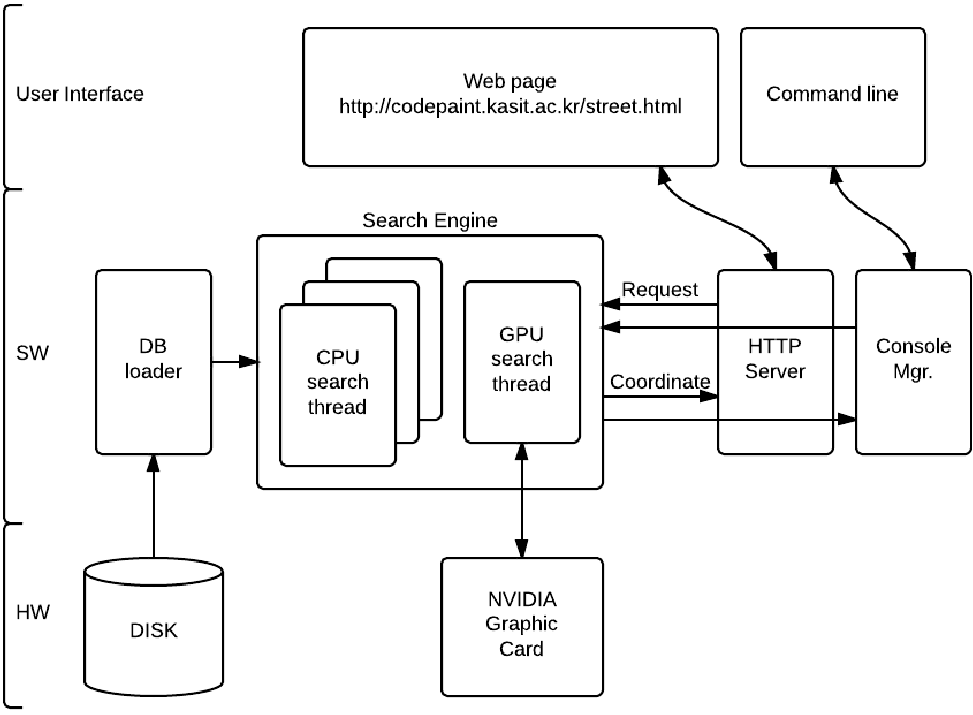
\includegraphics[scale=0.50]{figs/arch}
	\vspace{-0.1in}
	\ourcaption{Overall architecture of \name{}}
	\vspace{-0.1in}
	\label{fig:arch}
\end{figure}

\name{} is composed of DB loader module, search engine module and HTTP server module.
When the image search request arrives via HTTP server module, search engine module does vector matching between the input and database loaded by DB loader module.
The database, DB, which is consits of many pairs of geo-location and feature vector is generated befor running the \name{} by applying SURF to street view images.
The search engine module use both CPU and GPU resource to minimize the searching cost.
After the searching is finished, it notice the most probable geological location to the HTTP server module.
Then HTTP server generates HTML code and respond the request.

\oursubsection{DB Loader}
DB loader hides latency of reading DB file by dividing the DB into chunks and prefetching the next chunk to be used while the search engine is processing.
It has a large size, typically several GB, of ring buffer to read DB.
%It has a ring buffer and a large size of memory cache.


\textbf{Cache eviction policy:}
\note{TBD}

\oursubsection{Search Engine}
Search engine is the key component of \name{}.
When other modules such as HTTP server request searching to the search engnine, the request does not processed immediately.
Instead, it is enqueued to a request queue in the search engine and processed by FIFO order.
After searching, the search engine replies the request with only one geological location and its score which indicates how reliable the result is.

It maintains worker thread pool and distributes the searching job to them.
There is two types worker threads, one is using CPU and the other is using GPU.
Usually a search engine have CPU worker threads as many as the number of the machine's logical cores and GPU worker threads as many as the number of general purpose graphic cards.
Each worker thread requests a part of DB to the DB loader and process it repeatedly until the entire DB is processed.
After then, the result from each worker thread is merged by one of the worker thread.

\oursubsubsection{Score of Geological Locations}
Image searching with SURF results many geo-location candidates for a single input image.
We assume that the candidate which has many well-matched vectors is the most probable candidate.
SURF calculates ratio of best-fit distance and second-fit distance for each vector matching.
The best-fit distance is a minimum eucladian distance between a vector of needle and one of vectors of haystack.
The second-fit distance is the secondary minimum in same mannar.
If the ratio is higher than certain level, on the other words, best-fit distance is not very different from second-fit distance, it discards the matching.
We do not discard matching even though the ratio described above is not good, however, we calculate score for each vector matching,
$u = 1 - (best\_fit\ distance / second\_fit\ distance)$.
$u$ also means the uniqueness of the matching.
Score of candidates which have zero or more matched vectors is sum of $u$ of each vector matching.
The search engine selects a candidate with the highest score as a geo-location for the input image.

\oursubsubsection{Parallel Processing}

%\begin{figure}[!t]
%	\begin{separation}
%		\textbf{\em Merging} 
%		\vspace{-0.4cm}
%		\separator
%		\vspace{-0.2cm}
%		For two different search results from two different part of DB
%		\smallskip
%		\begin{compactitem}
%		\item[\bf Input:] $r_A$ and $r_B$
%		\item[\bf Output:] $r_M$
%		\end{compactitem}
%		\medskip
%		\begin{compactenum}[\sl 1.]
%		\item {\bf if } $r_A.best\_dist \le r_B.best\_dist$
%		\item \note{TBD}
%		\end{compactenum}
%
%		\vspace{-0.2cm}
%	\end{separation}
%	\caption{Algorithm description of merging}
%	\label{fig:merging}
%\end{figure}

SURF's vector matching algorithm is highly parallelizable since there is no data dependency between each vector matching.
The DB is usually splitted into many small pieces before searching and the splitted search result is merged into single one.
Result of each splitted piece of DB is calculated in an intermediate form to be merged with results from other pieces.
Hence our scoring algorithm requires second-fit distance of each vector matching so the intermediate result is consists of geo-location of best-fit vector, best-fit distance and second-fit distance.
The merged result have new best-fit distance and second-fit distance among all unmerged .
A score of vector matching is computed after all the merging is finished.

\oursubsubsection{GPU Worker}
Nvidia provides General Purpose GPU, GPGPU, and its programming environment, CUDA.
GPU is parallel computing resource separated from CPU.
We can boost up searching process by offloading some part of computation to GPU.
However, copying DB from memory to GPU via PCI bus involves long delay so GPU worker thread should minimize the overheady by requesting large enough portion of DB to DB loader.
%Caching the DB in graphic card memory can be helpful to avoid memory copy between main memory and graphic card memory.

\oursubsection{HTTP Server}
HTTP server module provides web interface to users over the internet.
It handles client's page request, search request and its attatched images.
It converts input images to a set of vectors by doing SURF and deliver it to the search engine module.
After searching, it serves result web page to the client.


\oursection{Implementation}

\oursubsection{DB Loader}
%DB loader is consist of circular ring buffer and large size of memory cache.
DB loader load DB file to large size of ring buffer it has.
It provides internal API for zero-copy read or write on the buffer to search threads.
{\tt acquire(void **ptr, int len)} requests a part of the buffer to read and {\tt release(void *ptr, int len)} releases the acquired part of buffer.
A search thread may hold a part of buffer while searching and releases it after the searching.
DB loader can load another part of DB after a search thread release the buffer it holds on.
Note that GPU search thread may release the buffer before finish searching because it does not need to hold buffer after copying the data to the GPU memory.
%It copies data from or to the buffer when write function or read function is called, respectively.
%In most of cases memcopy is unnecessary and can be replaced by zero-copy read operation.
%The zero-copy operation will be implemented later.
%Large size of memory cache is not implemented yet.
%So DB loader repeatedly reads the DB from disk even when sufficient memory is provided.

\oursubsection{Search Engine}
Search engine is designed to have thread pool of workers, each worker takes some portion of DB from DB loader, and result of each worker is merged together at last.
Unfortunately, current implementation is a bit inefficient.
A portion of DB read by DB loader is divided by 10 pieces and feeded to CPU search threads or GPU search threads one by one.
In CPU search function then spawns worker thread and divide its input to equal pieces for each worker thread.
In GPU search function copies its divided input to GPU and copy the result after processing.
As a result, 1 GB of the DB is divided into too small pieces, 30 MB, so sum of thread creation, data transfer to GPU and other overheads becomes hundreads of milli seconds which is not negligible.

\textbf{AVX:}
Advanced Vector Extension, AVX, is an extended instruction set of x86 provided by Intel to achieve instruction level data parallelism.
CPU can do at most 8 single-precision floating point calculation at once.
Calculating eucladian distance of two different feature vector can be done by only eight iterations of AVX instructions since each feature vector is consist of 64 single-precision floating point variables.

%\textbf{Highly efficient CUDA kernel:}
%Nvidia graphic cards expose L1 cache as shared memory to programmers.
%\note{TBD}

%\textbf{Cache-aware programming:}
%Typical Intel CPUs have 2 or 4 physical cores and 3 to 6 MB of L3 cache shared by all physical cores. \note{Should I delete this paragraph?}

\textbf{Queueing:}
Search engine handles simultaneously incoming requests so it provides circular queue of request and internal APIs for enqueueing.
When there are requests to be processed, they are processed in FIFO order and Search engine sleeps when the queue is empty.

\oursubsection{HTTP Server}

\begin{figure}[t]
	\centering
	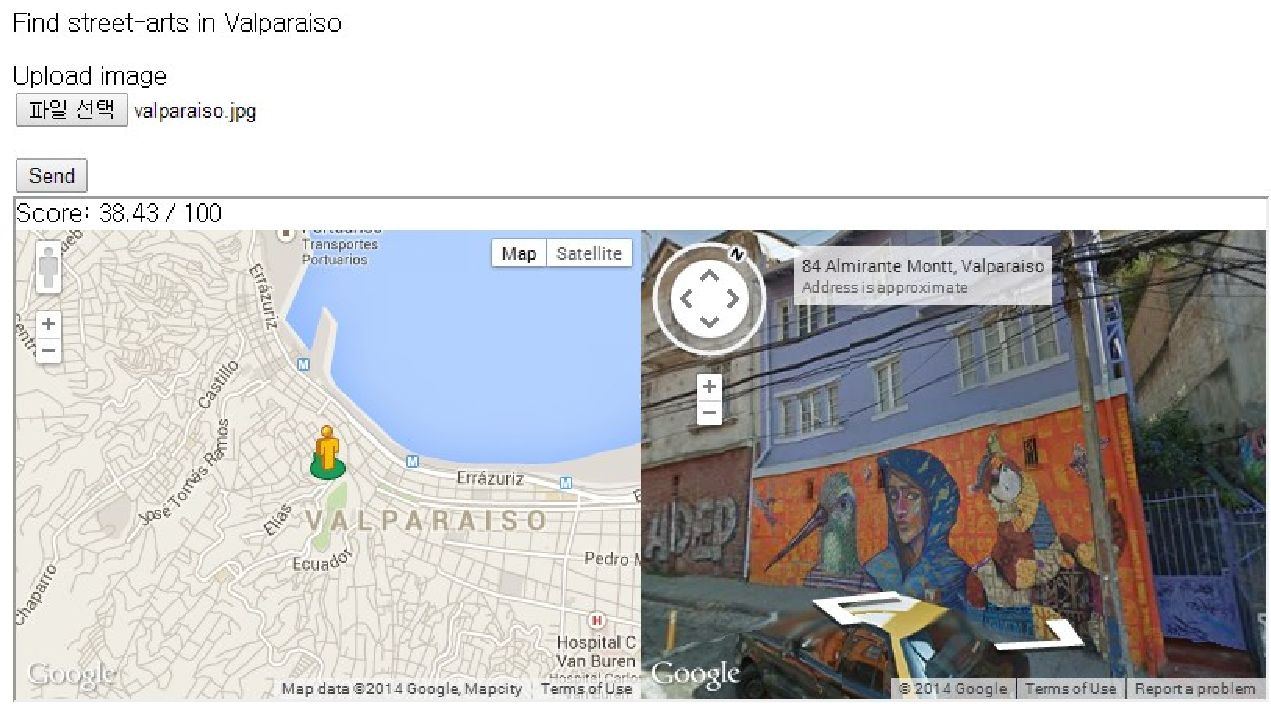
\includegraphics[scale=0.38]{figs/web_sample}
	\vspace{-0.1in}
	\ourcaption{Screen capture of search result web page}
	\vspace{-0.1in}
	\label{fig:web_sample}
\end{figure}

Functionality of HTTP server is divided by two, one is serving front page of the service which includes empty 'iframe' and the other is receive images from a client and update the 'iframe'.
The former is in charge of Nginx, an open source web server, and the latter is in charge of \name{}.
When the client connects to Nginx, it serves a static web page, 'street.html' which has upload button and empty 'iframe'.
When the client uploads an image file, it sends HTTP POST message which has the image file to the \name{}.
HTTP server of \name{} parses HTTP POST message, extract the image and write it to the disk.
Then the HTTP server read it from the disk, SURF it, extract feature vectors, enqueue it to the search engine, and sleep by 'select()' system call.
Limited APIs of OpenCV leads the unnecessary disk access.
Actual disk access may be avoided by using RAM disk.
HTTP server is waken up after the search engine finishes searching.
It sends response html web page, 'resp.html' which include matching score, Google maps and Google street views pointing the location of search result.
Figure~\ref{fig:web_sample} shows an example of the search result web page.


\oursection{Evaluation}
I have done some experiments to prove that \name{} speeds up image searching and finally lower the searching cost enough to serve the service on web.
\oursubsection{Searching Speed}


\oursubsection{Correctness}


\oursection{Conclusion}

I have presented \name{}, an image search server, which is fully utilizing CPU and GPU resources.
It speed up searching 38 times compare to single-threaded simple search program.


\oursection{Discussion}
%\oursubsection{DB Cache}
%\oursubsection{Fine-grained Crawling}
%\oursubsection{Scoring Algorithm}
\oursubsection{Grouping}

\textbf{Geological grouping:}

\textbf{Feature grouping:}
\oursubsection{Scaling Out to Distributed System}
\note{classifying the images}
\oursubsection{Removing Distortion from Street View}
\oursubsection{Caching The Search Result}


\bibliographystyle{unsrt}
\bibliography{report}

\end{document}

